\documentclass[UTF8,fontset=fandol,11pt]{ctexart}
\usepackage[a4paper,margin=24mm,headheight=15pt]{geometry}
\usepackage{amsmath,amssymb,amsthm,mathtools,bm}
\usepackage{enumitem,booktabs,longtable,array,pdfpages,fancyhdr,xcolor}
\usepackage[colorlinks=true,linkcolor=blue!45!black,urlcolor=blue!45!black]{hyperref}
\allowdisplaybreaks[2]
\setlength{\parindent}{2em}
\setlength{\parskip}{3pt}
\setlength{\emergencystretch}{3em}
\setlist{nosep,topsep=3pt}
\pagestyle{fancy}\fancyhf{}\fancyhead[L]{\small 分析学讲义习题解答}\fancyhead[R]{\small 第38--57讲}\fancyfoot[C]{\thepage}
\newcommand{\R}{\mathbb R}\newcommand{\C}{\mathbb C}\newcommand{\N}{\mathbb N}\newcommand{\Z}{\mathbb Z}\newcommand{\Q}{\mathbb Q}\newcommand{\T}{\mathbb T}
\newcommand{\dd}{\,\mathrm d}\newcommand{\eps}{\varepsilon}\newcommand{\ind}{\mathbf1}
\newcommand{\norm}[1]{\left\lVert#1\right\rVert}\newcommand{\abs}[1]{\left|#1\right|}\newcommand{\ip}[2]{\left\langle#1,#2\right\rangle}
\DeclareMathOperator{\supp}{supp}\DeclareMathOperator{\rank}{rank}\DeclareMathOperator{\Span}{Span}\DeclareMathOperator{\diag}{diag}\DeclareMathOperator{\Res}{Res}\DeclareMathOperator{\Ext}{Ext}
\newcommand{\problem}[2]{\subsection*{#1}\addcontentsline{toc}{subsection}{#1}\noindent\textbf{题干。}#2\par\smallskip\noindent\textbf{解答。}}
\newcommand{\fix}[1]{\par\noindent\textcolor{red!55!black}{\textbf{原文核对与修正。}#1}\par}
\newcommand{\skipnote}[1]{\par\noindent\textbf{依约不解的计算题。}#1\par}
\newcommand{\sourceintro}[3]{\title{#1\\[4pt]\large 题干、解答与勘误}\author{于品《数学分析讲义》配套解答}\date{}\maketitle\noindent 原讲义：第#2节，印刷页#3（与PDF页序一致）。题干按数学内容重排；完整原题页附于文末，含未解的传统计算题，供逐字核对。原文中的作业提交说明及引文不作为本项目的工作指令。\par 本文中的“正函数”均按非负函数理解。复内积约定对第一个变量线性。}
\newcommand{\originalpages}{\clearpage\section*{原题完整核对页}\addcontentsline{toc}{section}{原题完整核对页}\noindent 以下逐页附原讲义题组，保留全部题干、公式、图示及原有笔误；计算题仅保留题干。\clearpage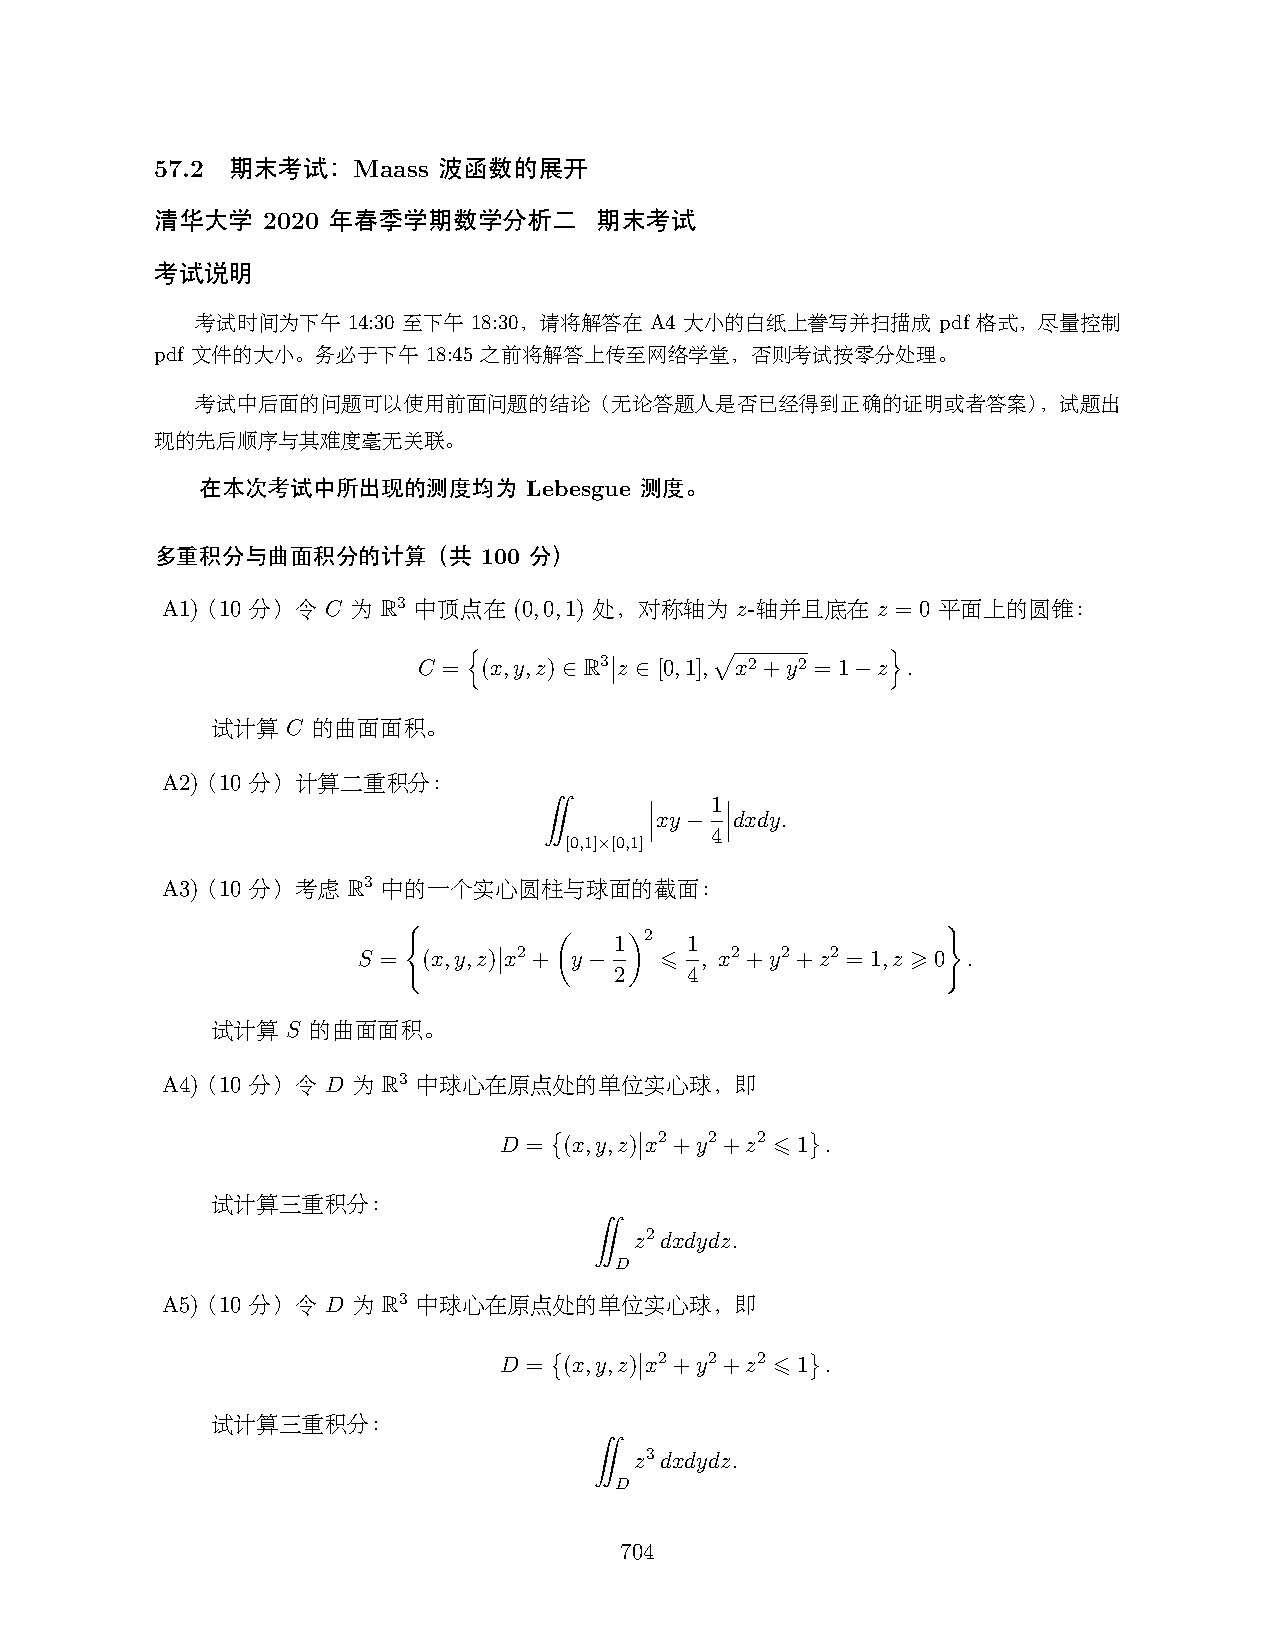
\includepdf[pages=-,pagecommand={\thispagestyle{empty}},scale=.94]{original.pdf}}

\begin{document}
\sourceintro{57.2 期末考试：正定函数与Maass波函数展开}{57.2}{704--708}
\section*{所用知识}
第43--57讲的积分求导、Fubini、Stokes、Fourier的$L^2$理论和Fejér逼近；第24讲常微分方程。$K_s$的渐近、二阶方程的全部解及其增长性在本文从积分定义推导，不引用特殊函数手册、分布理论或谱理论。
\section{第一部分的理论题}
\skipnote{A1--A7的圆锥面积、二重积分、球冠面积、三重积分及具体曲面通量计算全部不解。每题完整题干和公式见附录第704--705页。}
\problem{A8}{设$X=(X_1,X_2,X_3)$为$\R^3$上光滑散度零向量场，$S_R=\{|x|=R\}$。证明$I(R)=R^{-1}\int_{S_R}(xX_1+yX_2+zX_3)\dd\sigma$不依赖$R$。}
在$S_R$上外法向量为$x/R$，故$I(R)=\int_{S_R}X\cdot\nu\dd\sigma=\int_{B_R}\operatorname{div}X\dd x=0$。不但与半径无关，而且恒为零。若场仅在去原点域上光滑，则只能由环域散度定理得到半径无关，不一定为零；本题假设是全空间光滑。
\section{具有非负Fourier系数的连续函数}
对$2\pi$周期连续$f$，若每个有限数组$x_a\in\R,c_a\in\C$均满足$\sum_{a,b}c_a\overline{c_b}f(x_a-x_b)\ge0$，称$f$正定。该不等式也断言所得复数为实数。
\problem{B1}{若$f$为有限Fourier级数且所有系数非负，证明$f$正定。}
\[\sum_{a,b}c_a\overline{c_b}f(x_a-x_b)=\sum_k\widehat f(k)\abs{\sum_ac_ae^{ikx_a}}^2\ge0.\]
\problem{B2}{若连续$f$的全部Fourier系数非负，证明$f$正定。}
Fejér平均为有限级数，系数$(1-|k|/(N+1))_+\widehat f(k)$非负，所以由B1正定。Fejér平均一致收敛到$f$，对任一固定有限数组取极限即可。
\problem{B3}{若连续$f$正定，证明每个连续$g$都满足$\int_{-\pi}^\pi\int_{-\pi}^\pi f(x-y)g(x)\overline{g(y)}\dd x\dd y/(2\pi)^2\ge0$。}
取等分网格点$x_a$和$c_a=g(x_a)/m$，正定性给出每个二维Riemann和非负。被积函数连续，取$m\to\infty$得到积分，且极限为非负实数。
\problem{B4}{若连续$f$正定，证明每个$\widehat f(k)\ge0$。}
在B3取$g(x)=e^{-ikx}$。令$t=x-y$，利用周期性，对$x$的归一化积分为$\widehat f(k)$，外部$y$积分为$1$，故该系数非负。
\section{Maass波函数：定义与截面}
令$\mathbb H=\{(x,y):y>0\}$、$X_\eps=(0,1)\times(\eps,\infty)$。
\[\mathcal E=\{f:\mathbb H\to\C:f(x+1,y)=f(x,y),\ f|_{X_\eps}\in L^2(\dd x\dd y)\text{ 对每个 }\eps>0\},\]
\[\Delta_{\mathbb H}=y^2(\partial_x^2+\partial_y^2),\qquad \mathcal E_s=\{f\in C^2(\mathbb H)\cap\mathcal E:\Delta_{\mathbb H}f=(s^2-1/4)f\}.\]
\problem{M1}{对$f\in\mathcal E$，证明几乎每个$y>0$的$x\mapsto f(x,y)$属于$L^2(0,1)$。}
在每个$X_{1/j}$上对$|f|^2$使用Tonelli，截面积分几乎处处有限。取可数个$j$的异常集之并，便同时覆盖所有$y>0$。
\problem{M2}{对每个$k\in\Z$，证明$a_k(f,y)=\int_0^1f(x,y)e^{-2\pi ikx}\dd x$几乎处处有定义，且在每个$(\eps,\infty)$上属于$L^2(\dd y)$。}
由M1及长度为$1$的区间上的Cauchy--Schwarz可得绝对可积，且
\[|a_k(f,y)|^2\le\int_0^1|f(x,y)|^2\dd x.\]
对$y$积分得到所求界。异常截面上的系数可赋零；其可测性由Fubini参数积分给出。
\section{从积分定义研究K函数}
对$s\in\R,y>0$，定义$K_s(y)=\int_0^\infty e^{-y(u+u^{-1})}u^{s-1}\dd u$。
\problem{M3}{证明$K_s$良定义且光滑，并证明
\[K_s^{(n)}(y)=(-1)^n\int_1^\infty e^{-y(u+u^{-1})}(u^{s-1}+u^{-s-1})(u+u^{-1})^n\dd u.\]}
在$(0,1)$换元$u=1/v$得到$K_s=\int_1^\infty e^{-y(u+u^{-1})}(u^{s-1}+u^{-s-1})\dd u$，亦知$K_s=K_{-s}>0$。在$y\in[a,b]\subset(0,\infty)$上，任意阶导数的绝对值由$e^{-au}$乘一个固定幂增长函数控制，可积。因此反复积分求导得到公式及光滑性。
\problem{M4}{证明对每个$n\ge0$，$\lim_{y\to\infty}\sqrt y e^{2y}K_s^{(n)}(y)=(-2)^n\sqrt\pi$。}
用$u=e^t$写成$K_s^{(n)}(y)=\int_\R(-2\cosh t)^ne^{-2y\cosh t+st}\dd t$。再令$t=v/\sqrt y$，得到
\[\sqrt y e^{2y}K_s^{(n)}(y)=\int_\R(-2\cosh(v/\sqrt y))^n e^{-2y(\cosh(v/\sqrt y)-1)+sv/\sqrt y}\dd v.\]
逐点极限为$(-2)^ne^{-v^2}$。对$y\ge1$，$\cosh z-1\ge z^2/2$且$\cosh(v/\sqrt y)^n\le e^{n|v|}$，绝对值被$2^ne^{-v^2+(n+|s|)|v|}$控制，故控制收敛给出结论。此证明包含高阶导数的渐近，而不只函数本身。
\problem{M5}{令$Dh=y^2h''+yh'-4y^2h$，证明$DK_s=s^2K_s$，给出具体运算。}
置$h_y(t)=e^{-2y\cosh t}$，$w(t)=e^{st}$。有
\[\partial_th_y=-2y\sinh t\,h_y,\qquad\partial_t^2h_y=(-2y\cosh t+4y^2\sinh^2t)h_y.\]
另一方面$K_s'=\int(-2\cosh t)h_yw$、$K_s''=\int4\cosh^2t\,h_yw$，故
\begin{align*}
y^2K_s''+yK_s'-4y^2K_s
&=\int_\R[4y^2(\cosh^2t-1)-2y\cosh t]h_yw\dd t\\
&=\int_\R\partial_t^2h_y\,w\dd t
=-\int_\R\partial_th_y\,s w\dd t
=\int_\R h_y\,s^2w\dd t=s^2K_s.
\end{align*}
两次分部积分的边界项均为零，因为$e^{-2y\cosh t}$比任意$e^{-A|t|}$衰减更快；所有被积函数亦绝对可积。这给出全部代数与边界步骤。
\problem{M6}{若$h\in C^2(0,\infty)$满足$Dh=s^2h$，证明存在$c_1,c_2\in\C$使
\[h(y)=\left[c_1+c_2\int_0^y\frac{\dd r}{rK_s(r)^2}\right]K_s(y).\]}
令$h=vK_s$并代入M5，消去$v$本身项，得
\[y^2K_sv''+(2y^2K_s'+yK_s)v'=0,\quad (yK_s^2v')'=0.\]
因$K_s>0$，故$v'=c_2/(yK_s^2)$。还需验证题中零下限合法。若$s\ne0$，由$K_s=K_{|s|}$并在$u\in[1/y,2/y]$积分，$K_s(y)\ge c_s y^{-|s|}$于小$y$成立，所以$1/(yK_s^2)\le C y^{2|s|-1}$可积。若$s=0$，在$u\in[1,1/y]$积分得$K_0(y)\ge c\log(1/y)$，相应上界$C/[y\log^2(1/y)]$也可积。因此可从$0$积分，常数吸收入$c_1$。反向代入可验证每个此式都是解。
\problem{M7}{证明每个上述解的$\lim_{y\to\infty}\sqrt y e^{-2y}h(y)$存在，且极限为零当且仅当$h$为$K_s$的常数倍。}
令$J(y)=\int_0^y\dd r/(rK_s(r)^2)$。M4给出$K_s(y)\sim\sqrt\pi y^{-1/2}e^{-2y}$，因此$J'(y)\sim e^{4y}/\pi$，由l'Hôpital法则（或尾部积分夹逼）得$J(y)\sim e^{4y}/(4\pi)$。所以
\[\lim_{y\to\infty}\sqrt y e^{-2y}h(y)=\frac{c_2}{4\sqrt\pi}.\]
这对复常数同样成立，极限零恰等价于$c_2=0$，即$h=c_1K_s$。
\section{Fourier展开的刻画（以下$s>1$）}
\problem{M8}{对$f\in\mathcal E_s$和每个$(x,y)\in\mathbb H$，证明$\sum_{k\in\Z}a_k(f,y)e^{2\pi ikx}=f(x,y)$。}
固定$y$，$f(\cdot,y)$为$C^2$周期函数，两次分部积分给出$|a_k|\le C_y/k^2$，故级数绝对一致收敛。其和与$f$有相同Fourier系数，由Fejér唯一性相等。原文求和指标$n$与项中$k$混用，统一为$k$。
\problem{M9}{证明每个单模态$a_k(f,y)e^{2\pi ikx}$仍属于$\mathcal E_s$。}
在紧$y$区间可对$x$积分求两次$y$导数；对$x$两次分部积分，特征方程变为
\[y^2[a_k''(y)-(2\pi k)^2a_k(y)]=(s^2-1/4)a_k(y).\tag{1}\]
故单模态满足同一方程且$C^2$；周期性显然，$\mathcal E$中的$L^2$条件由M2得到。
\problem{M10}{若$k\ne0$，证明存在常数$a_k(f)$使$a_k(f,y)=a_k(f)y^{1/2}K_s(\pi|k|y)$。}
令$z=\pi|k|y$，$a_k(y)=y^{1/2}h(z)$。具体求导
\[a_k''=y^{-3/2}[-\tfrac14h+zh'+z^2h''],\]
代入(1)得$z^2h''+zh'-4z^2h=s^2h$。M6--M7说明其一般解由指数衰减分支$K_s$和指数增长分支组成。若增长分支系数非零，则$a_k(y)$的绝对值渐近于某个正常数乘$e^{2\pi|k|y}$，与M2的尾部$L^2$条件矛盾，所以只剩衰减分支。
\problem{M11}{证明存在常数$a_0(f)$使$a_0(f,y)=a_0(f)y^{1/2-s}$。}
令$k=0$，(1)为Euler方程，两个线性无关解为$y^{1/2+s},y^{1/2-s}$。第一项不能在$(\eps,\infty)$平方可积；第二项恰因$s>1$可积，所以只保留后者。
\problem{M12}{证明对每个$|z|<1$，$\sum_{k\ge1}(|a_k(f)|+|a_{-k}(f)|)z^k$收敛。}
固定$y>0$，$|a_{\pm k}(f,y)|\le\int_0^1|f(x,y)|\dd x=C_y$。M4给出$y^{1/2}K_s(\pi ky)\sim k^{-1/2}e^{-2\pi ky}$，故$|a_{\pm k}(f)|\le C_y'\sqrt k e^{2\pi ky}$。给定$r=|z|<1$，选择$y$足够小使$re^{2\pi y}<1$，即得到级数的绝对收敛。等价地，系数增长为任意小指数阶。
\problem{M13}{反之给定复常数$a_k$，假设每个$|z|<1$的$\sum_{k\ge1}(|a_k|+|a_{-k}|)z^k$收敛。证明
\[f(x,y)=a_0y^{1/2-s}+\sum_{k\ne0}a_ky^{1/2}K_s(\pi|k|y)e^{2\pi ikx}\]
定义$\mathcal E_s$中的函数。}
由假设对每个$\eta>0$都有$|a_{\pm k}|\le C_\eta e^{\eta k}$，因为收敛级数的单项有界。M4及连续性保证对每个$a>0$、整数$j\ge0$存在$C_{a,j}$使$|K_s^{(j)}(t)|\le C_{a,j}t^{-1/2}e^{-2t}$对$t\ge a$成立。故在任意紧条带$\eps\le y\le R$上，$x,y$任意有限阶导数的项由$Ck^Me^{-(2\pi\eps-\eta)k}$控制，选$\eta<2\pi\eps$得到一致绝对收敛。于是$f$光滑、周期，且可逐项使用M5得到特征方程。

剩下尾部$L^2$条件不可只用局部一致收敛替代。对$y\ge\eps$有$|y^{1/2}K_s(\pi ky)|\le C_\eps k^{-1/2}e^{-2\pi ky}$，所以
\[\int_\eps^\infty yK_s(\pi ky)^2\dd y\le C_\eps k^{-2}e^{-4\pi k\eps}.\]
在每个有限条带使用$x$方向Parseval，再对$y$用Tonelli，非零模态的总平方积分至多$C_\eps\sum_{k\ne0}|a_k|^2|k|^{-2}e^{-4\pi|k|\eps}<\infty$。常数模态的积分为$|a_0|^2\int_\eps^\infty y^{1-2s}\dd y<\infty$，因为$s>1$。因此$f\in\mathcal E$，完成所需的充要刻画。
\originalpages
\end{document}
